\documentclass{config/apuntes}

\title{Procesado y Manejo de Datos Masivos}
\author{Sandra Mingo Ramírez}
\date{2024/25}
\acronym{PRMDM}

\usepackage[all]{nowidow}
\usepackage{listing}
\usepackage{color}
\usepackage{tabularx}
\usepackage{multirow}
\usepackage{makecell}
\usepackage{amsmath}
\usepackage{array}

\definecolor{dkgreen}{rgb}{0,0.6,0}
\definecolor{gray}{rgb}{0.5,0.5,0.5}
\definecolor{mauve}{rgb}{0.58,0,0.82}

\lstset{
  frame=tb,
  aboveskip=3mm,
  belowskip=3mm,
  showstringspaces=false,
  columns=flexible,
  basicstyle={\small\ttfamily},
  numbers=none,
  numberstyle=\tiny\color{gray},
  keywordstyle=\color{blue},
  commentstyle=\color{dkgreen},
  stringstyle=\color{mauve},
  breaklines=true,
  breakatwhitespace=true,
  tabsize=3
}

\begin{document}

\begin{abstract}
En esta asignatura se aprenderán técnicas para procesar y manipular grandes volúmenes de datos utilizando programación y línea de comandos. Se abordará el manejo y análisis de formatos de datos comunes en bioinformática, como FASTA, GFF y GenBank, utilizando patrones que optimizan el uso de memoria y tiempo de ejecución, así como técnicas de programación paralela. Además, se realizarán operaciones avanzadas en bases de datos relacionales y no relacionales, y se explorará el acceso programático a bases de datos biomédicas online a través de sus APIs.
\end{abstract}

\pagestyle{plain}

\maketitle

\tableofcontents

%Se han invertido los temas y su orden: primero daremos herramientas de programación, y luego ya Linux
%Se trabaja en Linux principalmente, incluido Python (aunque funciona igual en Windows)
%08/10 - Gonzalo Martínez
\chapter{Procesado y manejo de datos masivos}
\section{Formatos de ficheros bioinformáticos}
Los formatos de fichero son en formato texto, y los principales son:
\begin{itemize}
\item \underline{FASTA}: guarda secuencia de nucleótidos o aminoácidos.
\item \underline{FASTQ}: conjunto de secuencias de nucleótidos leídas junto con sus puntuaciones de calidad
\item \underline{GFF/GTF}: formato de anotación de características del genoma
\item \underline{GenBank}: formato enriquecido para secuencias de nucleótidos o aminoácidos.
\end{itemize}

\subsection{FASTA}
Guarda una o varias secuencias de nucleótidos o aminoácidos. Se pronuncia como "fast A", que significa "fast all", siendo all cualquier alfabeto. Los archivos fasta pueden tener las siguientes extensiones:
\begin{itemize}
\item \textbf{.fasta, .fa}: extensión FASTA genérica
\item \textbf{.fna}: contiene secuencia de nucleótidos
\item \textbf{.faa}: contiene secuencia de aminoácidos
\item \textbf{.frn}: contiene secuencias de ARN no codificante
\end{itemize}

En la figura \ref{fig:fasta} se puede ver la estructura de un fichero FASTA. Cada secuencia consiste en una línea descriptiva seguida de las líneas que contienen la secuencia. La línea descriptiva cuenta con un símbolo > seguido del identificativo de la secuencia. Tras un espacio, se pone la descripción de la secuencia. En algunos casos, las secuencias se encuentran en mayúscula, en minúscula o en una mezcla de ambas. Por ello, se puede pasar toda la secuencia a mayúsculas o minúsculas con .upper() y .lower() respectivamente.

\begin{figure}[htbp]
\centering
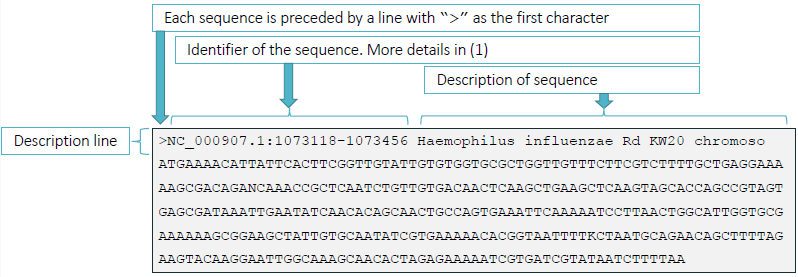
\includegraphics[width = \textwidth]{figs/fasta.png}
\caption{Anatomía de un fichero FASTA}
\label{fig:fasta}
\end{figure}

La secuencia se puede expandir por múltiples líneas, las cuales generalmente tienen unos 80 caracteres. No hay espacios en las líneas o líneas en blanco en una secuencia. Cada elemento de una secuencia se describe con un único carácter, y normalmente se escriben en mayúscula (aunque esto es una convención, no es estándar). No es recomendable utilizar guiones para representar gaps, ya que hay algunos programas que no los pueden manejar. Es mejor utilizar una N en el caso de secuencias de nucleótidos y X de aminoácidos (véase tabla \ref{tab:fasta-data}).

\begin{table}[htbp]
\centering
\begin{tabular}{l l l}
\multicolumn{3}{c}{\textbf{FASTA for genome data}}\\
A adenosine & C cytidine & G guanine \\
T thymidine & N A/G/C/T (any) & U uridine \\
K G/T (keto) & S G/C (strong) & Y T/C (pyrimidine) \\
M A/C (amino) & W A/T (weak) & R G/A (purine)\\
B G/T/C & D G/A/T & H A/C/T \\
V G/C/A & - gap & \\ \\ \hline \\
\multicolumn{3}{c}{\textbf{FASTA for protein data}}\\
A alanine & B aspartate/asparagine &  C cystidine\\
D aspartate & E glutamate & F phenylalanine\\
G glycine & H histidine & I isoleucine \\
K lysine & L leucine & M methionine \\
N asparagine & P proline & Q glutamine\\
R arginine & S serine & T threonine\\
U selenocysteine & V valine & W tryptophan\\
Y tyrosine & Z glutamate/glutamine & X any \\
* translation stop & - gap \\
\end{tabular}
\caption{Caracteres en los ficheros FASTA para datos genómicos y de proteínas.}
\label{tab:fasta-data}
\end{table}

\subsubsection{Parsear ficheros FASTA en Python}
En informática, parsear significa leer un fichero. Se pueden leer ficheros FASTA en Python de la siguiente forma:
\begin{lstlisting}[language=Python]
def readFasta(file):
    """ Reads all sequences of a FASTA file 
        returns a dictionary """  
    d = {}
    identifier = ''
    
    with open(file, 'r') as f:
        for linea in f:
            if linea[0] == ">": #alternativa: linea.startswith(">")
                if identifier != '':
                    d[identifier] = ''.join(d[identifier])
                descriptors = linea[1:].split()
                identifier = descriptors[0]
                #Alternativa: identifier = linea[1:linea.find(' ')]
                d[identifier] = []
                
            else:
                d[identifier].append(linea.strip('\n'))
        d[identifier] = ''.join(d[identifier])
    return d

readFasta("phix174/phix.fa")
\end{lstlisting}

\subsection{FASTQ}
Los ficheros FASTQ guardan secuencias de nucleótidos junto con las calidades.

Cada secuencia de un archivo FASTQ consta de 4 líneas. La primeras es la línea de descripción precedida de \@. Tiene un formato libre sin límite de longitud. A veces se coloca un identificador justo después de la \@. La segunda línea es la línea de secuencia, e incluye la secuencia propiamente dicha. Sigue normas y convenciones similares a las del fichero FASTA: normalmente en mayúsculas, sin espacios permitidos, etc. Esta línea podría estar envuelta en múltiples líneas como en un archivo FASTA. La siguiente es la línea que señala el final de la secuencia. Está marcada con el signo +. Puede ir seguida de la misma descripción dada en la primera línea. Sin embargo, es más sensato dejarla sólo con el '+' para reducir el tamaño de los ficheros. La última línea es la línea de puntuaciones de calidad: una secuencia codificada en caracteres con la calidad de las lecturas de la secuencia. Contiene un carácter por base. Los caracteres permitidos son como máximo ASCII 33-126 inclusive, que son todos imprimibles. Esta línea puede ser envuelta como en un archivo FASTA y su longitud total debe ser igual a la secuencia. Véase un ejemplo de un archivo FASTQ en la figura \ref{fig:fastq}.

\begin{figure}[htbp]
\centering
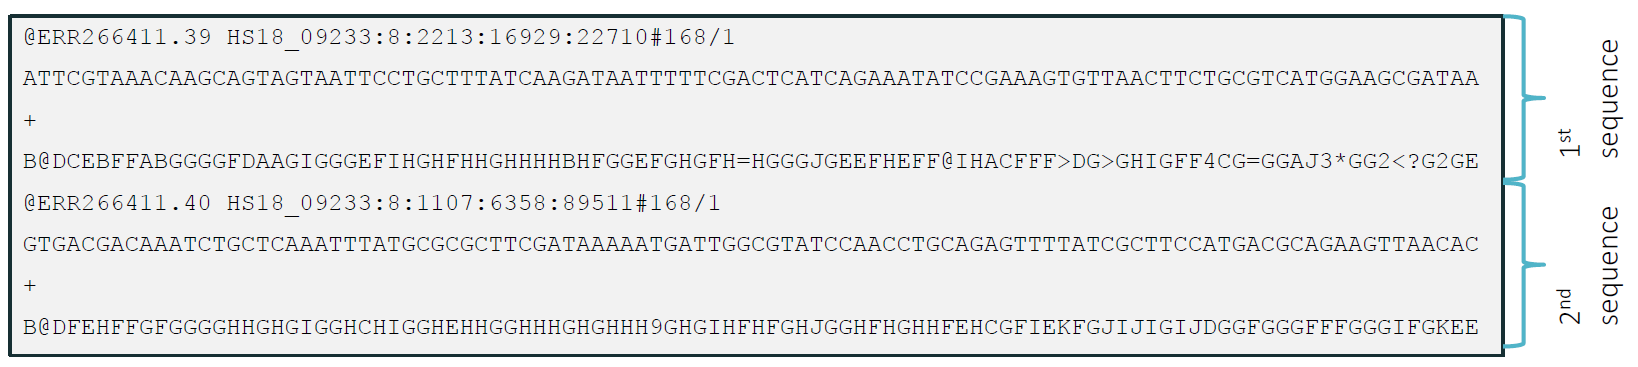
\includegraphics[width = \textwidth]{figs/fastq.png}
\caption{Anatomía de un fichero FASTQ}
\label{fig:fastq}
\end{figure}

Hay varias cuestiones que deben tenerse en cuenta al analizar un archivo FASTQ: Tanto el carácter \@ como + pueden aparecer en la línea con los índices de calidad. Pueden aparecer en la primera posición, por lo que hay que tener cuidado al utilizar grep o herramientas similares: por ejemplo \texttt{ \$> grep -v "[\@ +]" file.fastq} (Este comando para eliminar las líneas + y \@ no es una buena idea). En principio, tanto la secuencia como las puntuaciones de calidad pueden tener múltiples saltos de línea. El programa de análisis debería eliminar los saltos de línea. Para reducir los problemas de análisis sintáctico, la mayoría de las herramientas producen ahora archivos fastq en los que las secuencias y las puntuaciones de calidad se dan en una sola línea, posiblemente muy larga. Por lo tanto, cada secuencia tiene exactamente 4 líneas, lo cual es conveniente.

La codificación más utilizada para las puntuaciones de calidad es el formato Sanger o codificación Phred+33. Cada carácter codifica la calidad de la lectura, Q, que se define como:
$$Q = -10 \cdot log_{10} p$$
siendo p la probabilidad de error de la lectura. Esta puntuación de calidad se utiliza porque permite una interpretación fácil de la probabilidad (Q = 10, p = 1/10; Q = 20, p = 1/100; Q = 30, p = 1000) y porque permite una codificación en un único carácter ASCII. No obstante, no se puede guardar Q directamente como un carácter porque no todos son imprimibles. Por ello, se emplea la codificación Phred+33, que codifica el valor Q como:
$$Q = ord(chr) - 33$$
donde ord() convierte el carácter a su representación ASCII. Por ejemplo, el símbolo \@ tiene el código ASCII de 64, por lo que su Q sería de 31. Una p de 0 significa que es una lectura segura, mientras que una p de 1 indica que la lectura no es nada segura. Para calcular la p, se despeja la fórmula para que quede:
$$ p = 10^{-\frac{Q}{10}}$$

\textbf{Ejemplos:}
Para el carácter "~", el código ASCII es 126, por lo que su Q es $126-33 = 93$. En este caso, la p sería de $0,5 \cdot 10^{-10}$ .  Así, el carácter "!", cuyo ASCII es 33, tiene una Q de 0 y una p de 1. 

En este caso, como las letras en mayúscula y minúscula tienen un código ASCII diferente, no se puede pasar todo a mayúsculas o minúsculas como en FASTA.

\subsection{GFF: generic feature format}
Los ficheros GFF tienen un formato de texto sin formato para representar características genómicas. Cada característica está representada por nueve columnas separadas por tabuladores:
\begin{enumerate}
\item \underline{seqid}: id de la secuencia donde se localiza la característica. No se permiten espacios
\item \underline{source}: nombre del programa o algoritmo que ha generado esta característica.
\item \underline{type}: tipo de característica (region, gene, CDS, etc.)
\item \underline{start}: posición donde inicia la característica, su primera base
\item \underline{end}: posición donde finaliza la característica, su última base
\item \underline{score}: un valor flotante que indica la confianza en la característica. Si no se conoce, se pone un punto.
\item \underline{strand}: indica el sentido de la cadena, siendo + la cadena positiva y - la cadena negativa.
\item \underline{phase}: puede ser 0, 1 o 2 para CDS y un punto para todo lo demás. 
\item \underline{attributes}: Una lista de atributos de la característica en formato tag=value separados por punto y coma (;). Se permiten espacios en blanco en estas columnas, así como tabuladores y punto y coma si se escapan. Los atributos son:
\begin{itemize}
\item \textbf{ID}: El id de la característica. Debe ser único dentro del archivo gfffile. Tenga en cuenta que para las características no contiguas el id puede aparecer en varias líneas. Se considera una característica única
\item \textbf{Name}: Nombre de la característica. No es necesario que sea único.
\item \textbf{Parent}: Id del elemento padre. Indica la relación «parte de». Un elemento puede tener varios padres. En este caso, los identificadores se separan por comas.
\item \textbf{Note}: nota de texto libre
\item $\cdots$
\end{itemize}
\end{enumerate}

\begin{figure}[htbp]
\centering
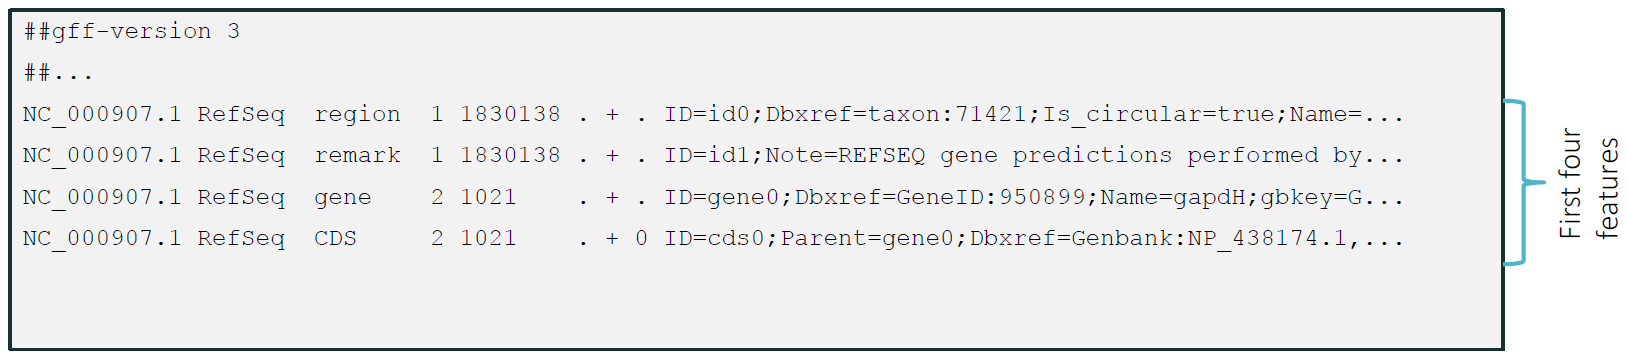
\includegraphics[width = \textwidth]{figs/gff.png}
\caption{Primeras columnas de un fichero GFF.}
\label{fig:gff}
\end{figure}

Hay varias cuestiones que deben tenerse en cuenta al analizar un archivo GFF: Las columnas sólo están separadas por tabuladores, pero se permiten espacios en blanco en algunos campos. Por tanto, hay que tener cuidado con grep y herramientas shell similares. Algunos caracteres se escapan en algunos campos, es decir, no queremos que los caracteres se interpreten como los caracteres que son. Esto ocurre con los puntos y coma y los espacios. Estos caracteres se escriben de otra forma; por ejemplo, un valor de a en punto y coma debe codificarse con \%3B. Para decodificar estos caracteres puede utilizar urllib. Además, una fila con triple almohadilla (\#\#\#) indica que se han resuelto todas las características multilínea hasta ese punto. Hay al menos una de estas líneas al final del fichero. Las líneas que empiezan por \# son comentarios. La región definida por los rasgos CDS incluye los codones de inicio y fin.

\begin{figure}[htbp]
\centering
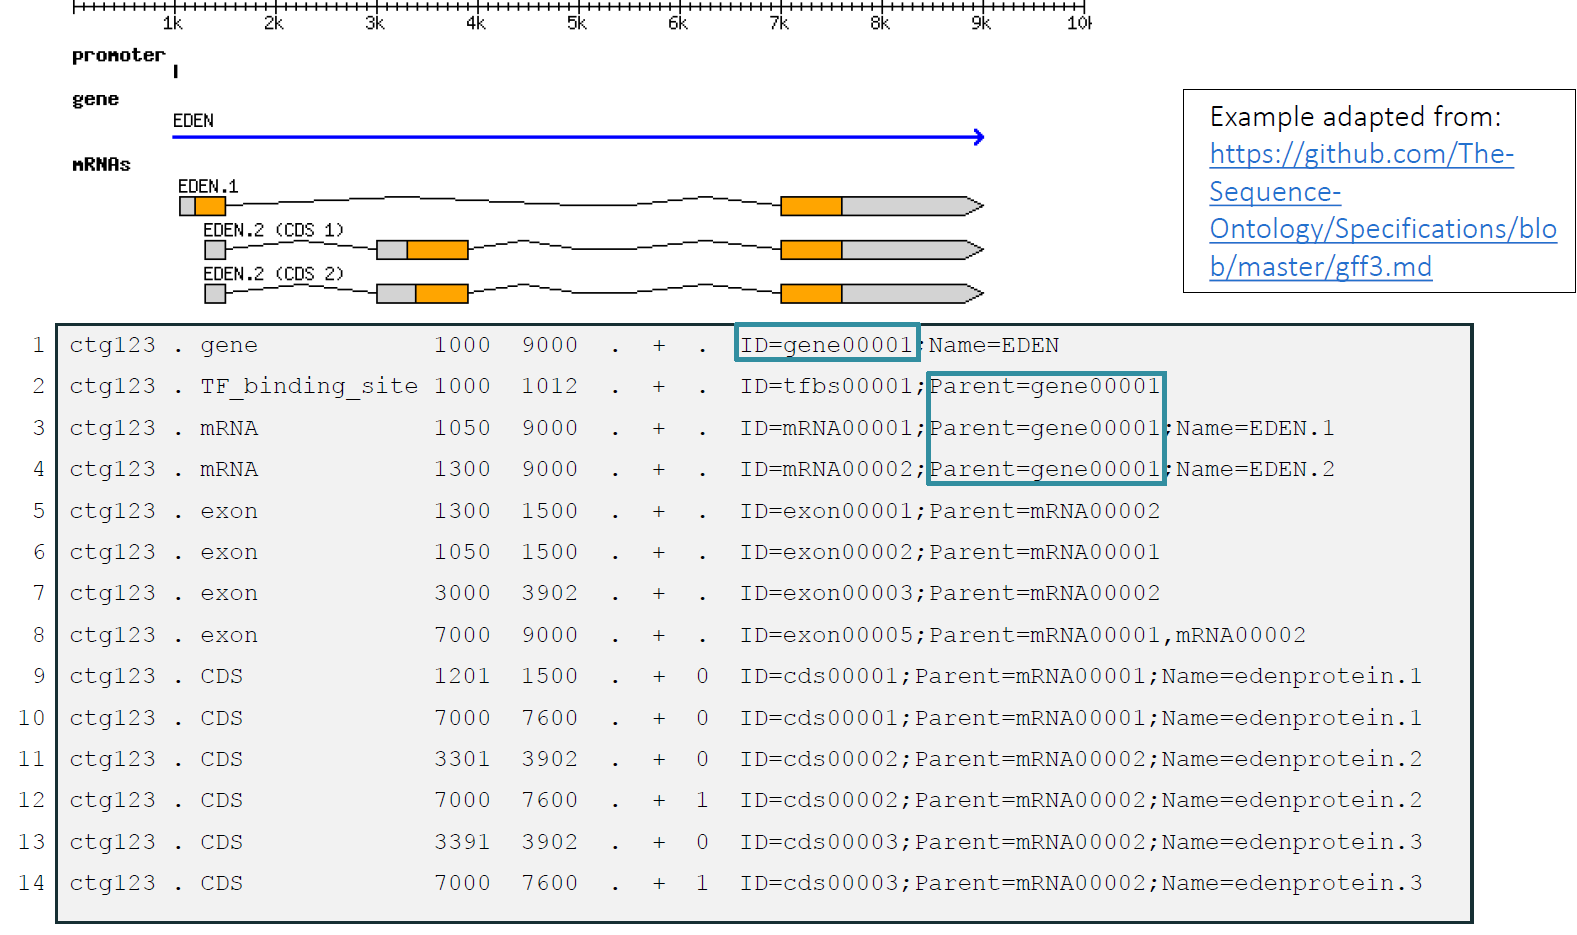
\includegraphics[width = \textwidth]{figs/gff-graph.png}
\caption{Ejemplo gráfico de una región genómica con el fichero GFF.}
\label{fig:gff-graph}
\end{figure}



\end{document}
